\documentclass{article}
\usepackage{graphicx,booktabs,geometry,amsmath,enumitem}
\geometry{a4paper,margin=1in}
\title{CS4532 Concurrent Programming \\ \large Take-Home Lab 1}
\author{Fernando T.H.L (210167E) \\ Gamage M.S (210176G)}
\date{\today}
\begin{document}
\maketitle
\section*{System Information}
\noindent
\begin{minipage}[t]{0.48\textwidth}
\subsection*{CPU}
\begin{itemize}[noitemsep,topsep=0pt]
  \item Model: Intel(R) Xeon(R) Processor @ 2.30GHz
  \item Vendor/Arch: GenuineIntel / x86-64
  \item Physical cores: 4
  \item Threads per core: 1
  \item Caches:
  \begin{itemize}[noitemsep,topsep=0pt,leftmargin=*]
    \item L1i: 128 KiB (4 instances)
    \item L1d: 128 KiB (4 instances)
    \item L2:  1 MiB (4 instances)
    \item L3:  45 MiB (1 instance)
  \end{itemize}
\end{itemize}
\subsection*{Memory / NUMA}
\begin{itemize}[noitemsep,topsep=0pt]
  \item Total (kB): 8150140
  \item NUMA nodes: 1
  \item THP: madvise
  \item Swap total (kB): 0
\end{itemize}
\end{minipage}
\hfill
\begin{minipage}[t]{0.48\textwidth}
\subsection*{Operating System}
\begin{itemize}[noitemsep,topsep=0pt]
  \item Distro: Ubuntu 24.04.2 LTS
  \item Kernel: 6.8.0
  \item Logical CPUs: 4
\end{itemize}
\subsection*{Toolchain}
\begin{itemize}[noitemsep,topsep=0pt]
  \item Compiler: gcc (Ubuntu 13.3.0-6ubuntu2~24.04) 13.3.0
  \item make: GNU Make 4.3
  \item glibc: glibc 2.39
  \item libpthread (NPTL): NPTL 2.39
  \item Python: 3.12.11
  \item pandas: 2.3.2
  \item matplotlib: 3.10.6
\end{itemize}
\end{minipage}
\section*{Approach}
We implemented a singly linked list supporting:
\begin{itemize}[noitemsep,topsep=0pt]
  \item \texttt{Member}
  \item \texttt{Insert} (unique keys only)
  \item \texttt{Delete}
\end{itemize}
Three variants were tested:
\begin{itemize}[noitemsep,topsep=0pt]
  \item Serial (no locks)
  \item Pthreads + single mutex
  \item Pthreads + single read--write lock
\end{itemize}
Initialization: $n=1000$ unique keys in $[0, 2^{16}-1]$.
Workloads: $m=10000$ operations with given fractions, distributed across $T \in \{1,2,4,8\}$ threads.
Timing measures only the $m$-operations region, not initialization.
\newpage

\section*{Experiment Report (Overview Tables)}
\subsection*{Case 1: n=1000, m=10000, m\_member=0.99, m\_insert=0.005, m\_delete=0.005}
\begin{table}[h!]
\centering
\begin{tabular}{cccc}
\toprule
\textbf{Threads} & \textbf{Serial (s)} & \textbf{Mutex (s)} & \textbf{RW-lock (s)} \\
\midrule
1 & 0.0096 $\pm$ 0.0003 & 0.0109 $\pm$ 0.0006 & 0.0109 $\pm$ 0.0008 \\
2 & 0.0100 $\pm$ 0.0003 & 0.0324 $\pm$ 0.0058 & 0.0132 $\pm$ 0.0008 \\
4 & 0.0095 $\pm$ 0.0004 & 0.0304 $\pm$ 0.0007 & 0.0164 $\pm$ 0.0021 \\
8 & 0.0100 $\pm$ 0.0005 & 0.0345 $\pm$ 0.0012 & 0.0193 $\pm$ 0.0011 \\
\bottomrule
\end{tabular}
\caption{Summary of results for Case 1.}
\label{tab:case1}
\end{table}
\subsection*{Case 2: n=1000, m=10000, m\_member=0.90, m\_insert=0.05, m\_delete=0.05}
\begin{table}[h!]
\centering
\begin{tabular}{cccc}
\toprule
\textbf{Threads} & \textbf{Serial (s)} & \textbf{Mutex (s)} & \textbf{RW-lock (s)} \\
\midrule
1 & 0.0197 $\pm$ 0.0005 & 0.0207 $\pm$ 0.0006 & 0.0211 $\pm$ 0.0006 \\
2 & 0.0199 $\pm$ 0.0004 & 0.0420 $\pm$ 0.0050 & 0.0812 $\pm$ 0.0075 \\
4 & 0.0206 $\pm$ 0.0007 & 0.0470 $\pm$ 0.0020 & 0.0925 $\pm$ 0.0100 \\
8 & 0.0212 $\pm$ 0.0013 & 0.0510 $\pm$ 0.0028 & 0.0879 $\pm$ 0.0117 \\
\bottomrule
\end{tabular}
\caption{Summary of results for Case 2.}
\label{tab:case2}
\end{table}
\subsection*{Case 3: n=1000, m=10000, m\_member=0.50, m\_insert=0.25, m\_delete=0.25}
\begin{table}[h!]
\centering
\begin{tabular}{cccc}
\toprule
\textbf{Threads} & \textbf{Serial (s)} & \textbf{Mutex (s)} & \textbf{RW-lock (s)} \\
\midrule
1 & 0.0676 $\pm$ 0.0018 & 0.0664 $\pm$ 0.0022 & 0.0674 $\pm$ 0.0018 \\
2 & 0.0644 $\pm$ 0.0018 & 0.0992 $\pm$ 0.0073 & 0.1673 $\pm$ 0.0047 \\
4 & 0.0651 $\pm$ 0.0017 & 0.1144 $\pm$ 0.0084 & 0.1835 $\pm$ 0.0104 \\
8 & 0.0653 $\pm$ 0.0023 & 0.1301 $\pm$ 0.0025 & 0.2136 $\pm$ 0.0107 \\
\bottomrule
\end{tabular}
\caption{Summary of results for Case 3.}
\label{tab:case3}
\end{table}
\paragraph{Sampling/Confidence}
For Case 1, the worst relative CI was 15.54%, which exceeds the 5% target.
For Case 2, the worst relative CI was 11.67%, which exceeds the 5% target.
For Case 3, the worst relative CI was 6.44%, which exceeds the 5% target.
The target of a 5% relative CI was not met for one or more configurations, suggesting more samples are needed.
\newpage
\section*{Case Analyses with Plots}
\subsection*{Case 1: Read-Heavy Workload}
\begin{figure}[h!]
\centering
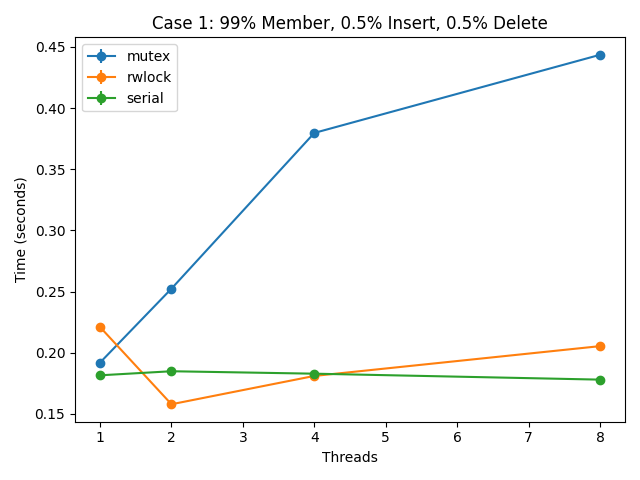
\includegraphics[width=0.9\textwidth]{report/graphs/case1_plot.png}
\caption{Average time vs. threads for Case 1.}
\label{fig:case1}
\end{figure}
\paragraph{Analysis}
As shown in Table~\ref{tab:case1} and Figure~\ref{fig:case1}, at 1 thread, serial is fastest (0.0096s) vs mutex (0.0109s) and rw-lock (0.0109s).
From 1 to 8 threads, mutex changes by 217.12% and rw-lock by 76.90%.
At 8 threads, rw-lock is 1.79x faster than mutex.
This workload is read-heavy (99% member operations), which explains the significant performance advantage of the rw-lock, as it allows for concurrent reads.
\newpage
\subsection*{Case 2: Balanced Workload}
\begin{figure}[h!]
\centering
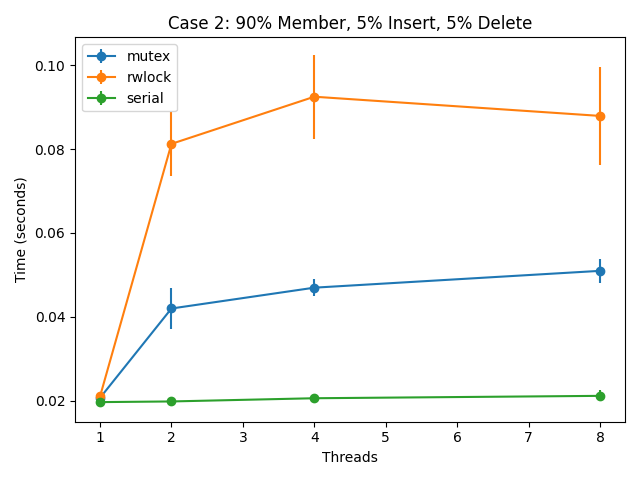
\includegraphics[width=0.9\textwidth]{report/graphs/case2_plot.png}
\caption{Average time vs. threads for Case 2.}
\label{fig:case2}
\end{figure}
\paragraph{Analysis}
As shown in Table~\ref{tab:case2} and Figure~\ref{fig:case2}, at 1 thread, serial is fastest (0.0197s) vs mutex (0.0207s) and rw-lock (0.0211s).
From 1 to 8 threads, mutex changes by 146.05% and rw-lock by 317.48%.
At 8 threads, rw-lock is 0.58x faster than mutex.
With a higher write fraction (10%), the advantage of rw-lock diminishes. The data suggests that for this particular workload and system, the overhead of the rw-lock is greater than its benefit from concurrent reads.
\newpage
\subsection*{Case 3: Write-Heavy Workload}
\begin{figure}[h!]
\centering
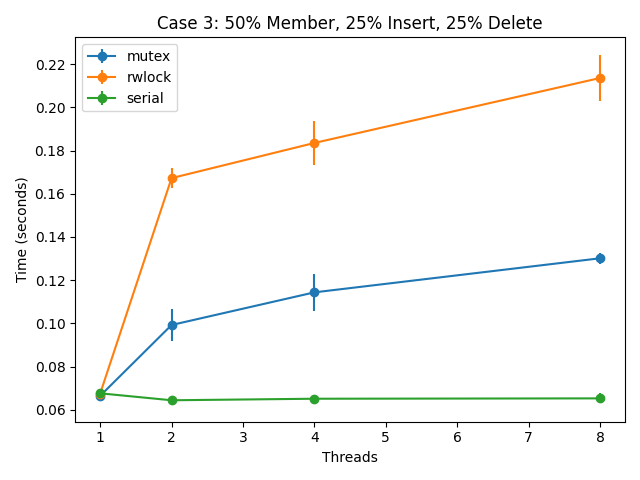
\includegraphics[width=0.9\textwidth]{report/graphs/case3_plot.png}
\caption{Average time vs. threads for Case 3.}
\label{fig:case3}
\end{figure}
\paragraph{Analysis}
As shown in Table~\ref{tab:case3} and Figure~\ref{fig:case3}, at 1 thread, serial is fastest (0.0676s) vs mutex (0.0664s) and rw-lock (0.0674s).
From 1 to 8 threads, mutex changes by 95.90% and rw-lock by 216.70%.
At 8 threads, rw-lock is 0.61x faster than mutex.
In this write-heavy scenario (50% insert/delete), both locking strategies suffer from contention as writes are serialized. The rw-lock's performance is worse than the mutex, indicating that its more complex logic adds significant overhead that is not offset by parallelism in read operations.
\newpage
\begin{figure}[h!]
\centering
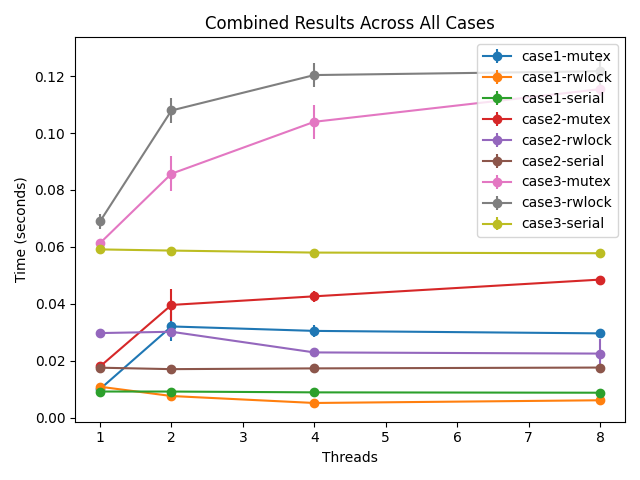
\includegraphics[width=0.8\textwidth]{{report/graphs/combined_plot.png}}
\caption{{Combined view across all cases and implementations.}}
\label{fig:combined}
\end{figure}
\section*{Conclusion}
Results align with expectations: the serial baseline dominates at T=1 (no lock overhead).
Read-heavy workloads: rwlock outperforms mutex via concurrent readers.
Write-heavier workloads: rwlock advantage shrinks; both converge due to writer serialization; parallel versions can underperform serial when contention dominates.
Scaling saturates near core count due to contention and scheduling overhead.
The $\pm$5% @ 95% CI target was not satisfied overall; it is advised to increase samples.
\end{document}